\chapter{Introduction}
\label{chp:introduction}

Autonomous cars have the potential to revolutionize transportation by providing mobility to a broad range of people. 
These vehicles will (a) increase the independence of those who are incapable of driving, (b) reduce the number of road accidents caused by driver negligence, and (c) reduce both road congestion and pollution by optimising routes and driving style. 
These are just a few ways in which autonomous cars are expected to impact our daily lives \cite{klaver}. 

However, there are numerous challenges to the large scale deployment of road-going autonomous cars. 
In particular, public roads are an unpredictable environment, and autonomous cars face a wide variety of scenarios which are difficult to program for.
There are many edge cases which will require the vehicle to not only respond quickly, but also operate at its handling limits to ensure the safety of its occupants.
An example of such a scenario is avoiding a collision \cite{Barab_s_2017}. 

The emergence of autonomous racing as a research field stems from the need to design autonomous driving solutions that address these edge cases.
The similarity of racing and road-going scenarios allows racing be used as a platform to develop autonomous road-going driving algorithms \cite{Weiss2020a}.

\section{Autonomous racing background}

As with algorithms intended to be applied to the road-going case, the goal in autonomous racing is to develop driving algorithms that convert sensor data into actuator commands.
However, unlike road-going scenarios, racing cars must travel as fast as possible around the track in a safe manner to be competitive.

The two objectives of of lap time and safety are juxtaposed.
This is because the faster a vehicle travels, the closer it is to its handling limit.
The requirements to develop algorithms that optimise for conflicting objectives and control vehicles at their handling limits makes autonomous racing an interesting and challenging problem to solve.
Furthermore, the requirement for vehicle safety at the handling limit make autonomous racing a suitable proxy for road-going edge cases.

The applicability of racing to road-going scenarios has led to the increasing popularity of autonomous racing leagues.
These racing leagues provide a competitive environment for teams to design and improve driving algorithms by providing clear evaluation metrics of lap time and safety, which is usually measured as number of track boundary collisions \cite{Betz2021}. 
Furthermore, the controlled nature of racing (e.g., there are no pedestrians and the number of cars on track is specified) creates safe environments for deploying new driving algorithms.
 
F1tenth (i.e., our chosen racing platform) achieves a safe and convenient development environment by specifying the use of a miniature remote controlled (RC) car chassis as the basis for the vehicle platform.
Since RC cars are cheap and relatively easy to modify, it is relatively easy to partake in F1tenth compared to other racing leagues.
An example of an F1tenth racing league standard vehicle is shown in Figure \ref{fig:f1tenth_car}.

\begin{figure}[htb]
\centering
  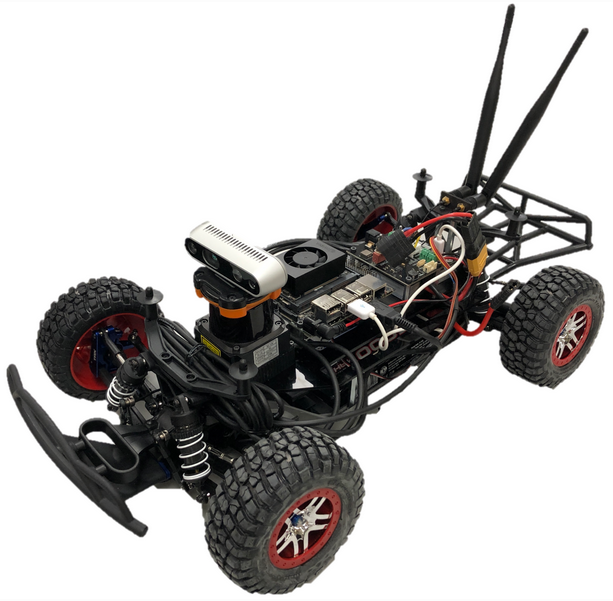
\includegraphics[width=.4\textwidth]{contents/chapt1/figs/f1tenth_car.png}
  \captionof{figure}[The F1tenth standard racecar]{The F1tenth standard vehicle, built on the chassis of a miniature RC car \cite{f1tenth}.}
  \label{fig:f1tenth_car}
\end{figure}


\section{Research motivation}

A recent breakthrough in autonomous racing was the introduction of learning-based solutions for vehicle control.
Learning-based solutions are commonly implemented within an end-to-end architecture, whereby a neural network is trained to map sensor data directly to actuator commands.
In particular, deep reinforcement learning (DRL) techniques have shown state of the art results in a variety of scenarios, including time trial and multi-vehicle racing \cite{Fuchs2021, Song2021}.

% DRL is a subfield of machine learning that considers the problem of optimising a computational agent to maximise a scalar reward signal through direct interaction with an environment.
% It is a powerful technique that is able to learn non-trivial behaviour from complex cost formulations for systems with non-linear dynamics \cite{Plaat_2022}.  

Although the results from end-to-end research efforts are promising, most applications are still limited to simulation due to the difficulty of deploying algorithms on physical hardware.
A large part of the difficulty is that DRL techniques rely on an assumed vehicle dynamics model to train the neural network.
However, this vehicle model is only an approximation of the real system dynamics. 
Discrepancies always exist between the simulated and actual vehicle dynamics due to the difficulty of measuring the model parameters \cite{Hewing2018}. 
These model inaccuracies cause a degradation in algorithm performance during physical deployment that can have catastrophic consequences.
This is known as the \emph{sim2real} gap \cite{Ivanov2020}.

% Research efforts into addressing the sim2real gap in learning-based approaches have largely been limited to modifying the training process to account for vehicle model uncertainty.
% For example, sim2real best practices include randomising vehicle model parameters during training, or retraining the neural network after deployment \cite{Zhou2020}.

A promising method to address the sim2real issues of current learning-based solutions is to include ideas from classical approaches. 
Classical architectures decouple the driving task into a series of modules with specific functions.
The task of planning a desired path and velocity profile (i.e., trajectory planning), and ensuring that the vehicle follows that trajectory (i.e., control) are handled separately. 
Well designed control algorithms allow classical approaches to overcome the sim2real gap by minimising the the error between the actual and planned trajectory \cite{Betz2021}. 

Approaches that synthesise classical and end-to-end architectures are known as partial end-to-end.
These approaches utilise the modularised structure of the classical architecture, but combine or replace modules with a neural network \cite{Weiss2020}.
Thus, partial end-to-end approaches leverage the reliability provided by the structure of classic approaches while benefitting from the heuristic nature of learning algorithms.
However, there are relatively few research efforts related to this architecture.
Furthermore, the use of this architecture to address the sim2real gap remains unexplored.


% In particular, a promising partial end-to-end approach to address the sim2- real gap within current learning-based solutions for autonomous racing is to use a DRL agent for trajectory prediction, in conjunction with a set of classical controllers for trajectory tracking \cite{Betz2021}.
% This architecture can benefit from the heuristic nature of the DRL agent to create a trajectory, while also leveraging classical controllers to increase robustness against modelling errors associated with practical hardware deployment.
% However, there are relatively few research efforts related to this architecture.
% Furthermore, the use of this architecture to address the sim2real gap remains unexplored.


%\begin{figure}[!htb]
%\centering
%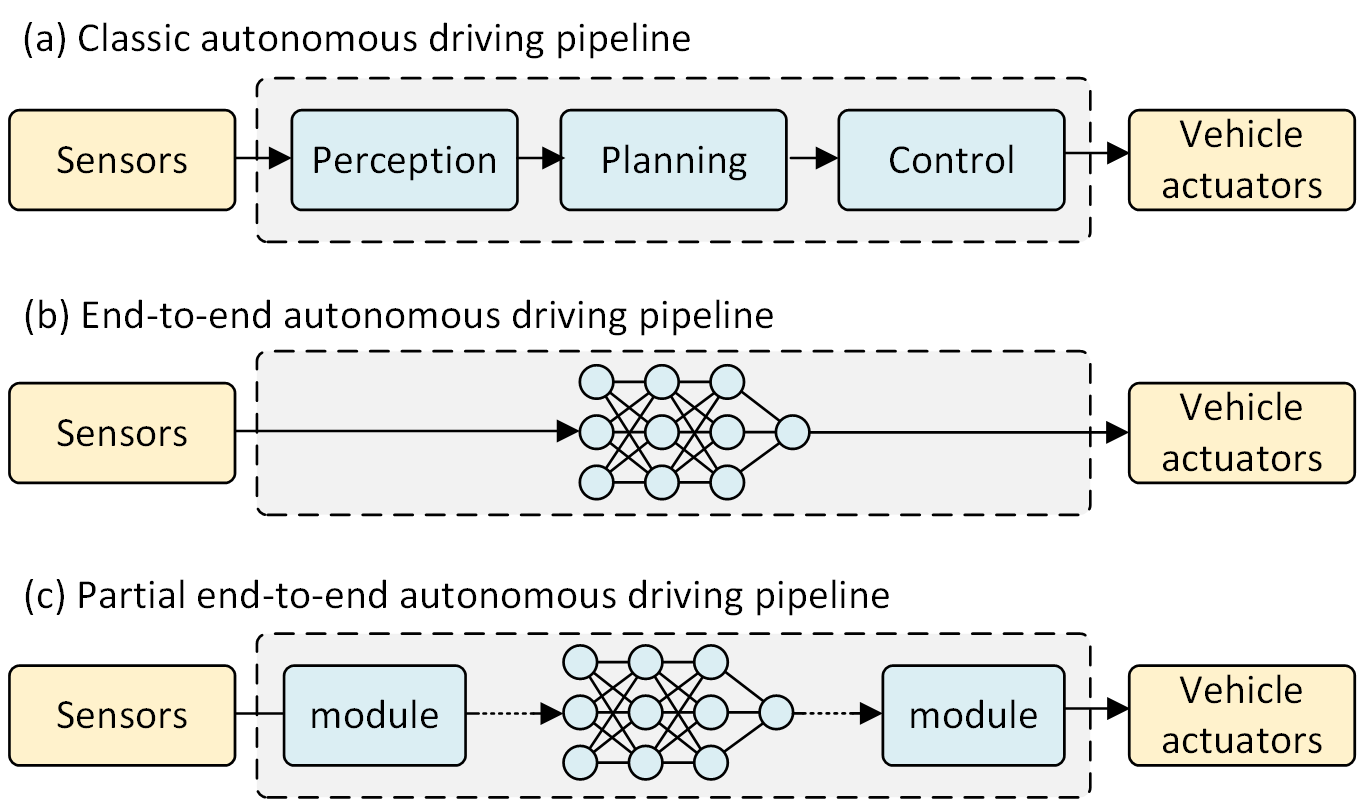
\includegraphics[width=\textwidth*8/10]{contents/chapt1/figs/architecture_comparisons.png}
%\caption[A comparison of the commonly used driving software architectures]{A comparison of the commonly used driving %software architectures.}
%\label{fig:architecture_comparison}
%\end{figure}

% \begin{figure}[htb!]
%     \centering
%     \begin{subfigure}[htb!]{\textwidth}
%         \centering
%         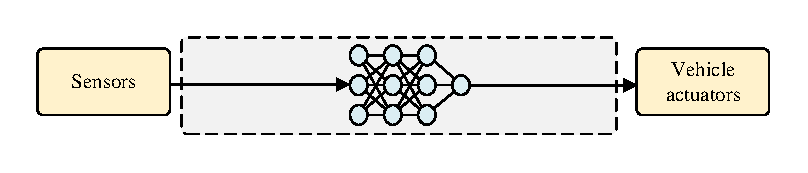
\includegraphics{contents/chapt1/figs/end_to_end.pdf}
%         \caption[The end-to-end pipeline]{The end-to-end pipeline.}
%         \label{fig:intro_ete}
%     \end{subfigure}
%     \hfill
%     \begin{subfigure}[htb!]{\textwidth}
%         \centering
%         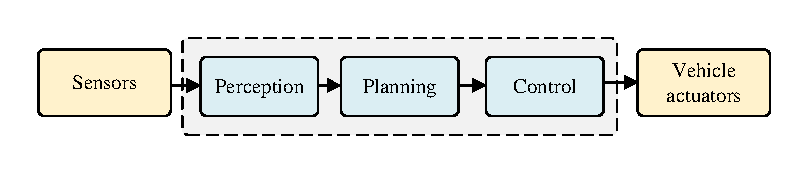
\includegraphics{contents/chapt1/figs/classic.pdf}
%         \caption[The classic pipeline]{The partial end-to-end pipeline.}
%         \label{fig:intro_classic}
%     \end{subfigure}
%     \hfill
%     \begin{subfigure}[htb!]{\textwidth}
%         \centering
%         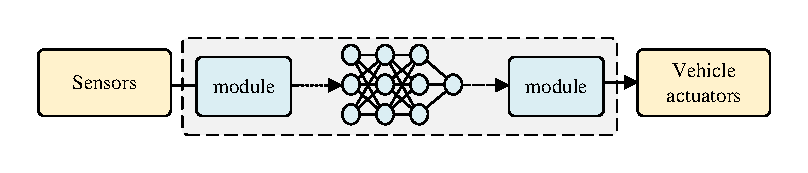
\includegraphics{contents/chapt1/figs/partial_end_to_end.pdf}
%         \caption[The partial end-to-end pipeline]{The partial classic pipeline.}
%         \label{fig:intro_pete}
%     \end{subfigure}
%     \hfill
%     \caption[A comparison of the commonly used driving software architectures]{A comparison of the commonly used driving software architectures.}
% \label{fig:architecture_comparison}
% \end{figure}

\section{Project aims and objectives}\label{sec:objectives}

The aim of this project is to investigate partial end-to-end autonomous driving software architectures for the task of autonomously racing around a track. 
We specifically aim to use the partial end-to-end architecture to address issues with typical learning-based (i.e., end-to-end) approaches, namely reliability and robustness to model inaccuracies. Our objectives are therefore:
\begin{enumerate}
    \item Investigate the literature regarding current partial end-to-end autonomous racing algorithms
    \item Identify a suitable configuration of the partial end-to-end architecture to address sim2real problems
    \item Develop a partial end-to-end autonomous driving algorithm
    \item Benchmark partial end-to-end against end-to-end techniques without model inaccuracies
    \item Benchmark partial end-to-end against end-to-end techniques with model inaccuracies
\end{enumerate}

\section{Solution overview and contributions}

We developed a partial end-to-end architecture whereby a DRL agent is used as a short-term trajectory planner.
The trajectory that the agent outputs consists of a path and desired velocity, which are tracked using a pure pursuit steering controller, and a proportional controller respectively.
This architecture benefits from the heuristic nature of the DRL agent to create a trajectory, while also leveraging classical controllers to increase robustness against modelling errors associated with practical hardware deployment.
% Our investigations were performed on a custom F1tenth simulator.

Our investigation into the performance of the partial end-to-end architecture in the absence of modelling errors revealed that it significantly outperformed end-to-end solutions in terms of time taken to train the agent.
Furthermore, partial end-to-end agents completed laps faster than end-to-end agents after training, thus operating closer to their handling limits.

When model inaccuracies were considered, the gap in performance between the partial end-to-end and fully end-to-end systems increased.
Our partial end-to-end system proved more robust against errors in mass, tire cornering stiffness and road surface friction coefficients than fully end-to-end systems.
Furthermore, our partial end-to-end system was able to reliably repeat laps, whereas an end-to-end system behaved erratically when modelling errors were significant.


% A partial end-to-end framework for reinforcement learning was developed using simulated F1tenth racing as a platform.
% We used a neural network to repeatedly output a path and velocity, which was tracked using a pure pursuit path tracking controller and a proportional controller, respectively.
% The partial end-to-end system showed similar performance as the end-to-end system under conditions with no model inaccuracy.
% However, our system proved more robust to simulated model-inaccuracies than the end-to-end system.
% In particular, a change in tire friction significantly deteriorated the performance of the end-to-end system, resulting in frequent collisions with the track boundary. 
% In comparison, our partial end-to-end system had fewer track boundary collisions.


\section{Document outline}
\label{sec:outline}

Chapter \ref{chp:litreview} constitutes an overview of the existing approaches to solving the autonomous racing problem in literature. 
% We briefly discuss solutions from the classic pipeline and end-to-end pipelines, before reviewing partial end-to-end approaches. 
% The core concepts of reinforcement learning are then discussed in Chapter \ref{chp:reinforcement_learning}.
We follow the with a description of how we modelled and simulated the racing problem in Chapter \ref{chp:modelling}.
Our end-to-end baseline agent is described in Chapter \ref{chp:end_to_end_autonomous racing}.
Our own work on the  partial end-to-end architecture for autonomous racing is presented in Chapter \ref{chp:partial_end_to_end_autonomous_racing}.
In Chapter \ref{chp:racing}, we consider racing in settings were the vehicle model used for training is inaccurate.
Finally, the thesis concludes with a summary of our findings and proposal for future work in Chapter \ref{chp:conclusion}.

